\documentclass{article}
\usepackage[english]{babel}
\usepackage[margin=2.5cm]{geometry}
\usepackage{graphicx}
\usepackage{float}
\usepackage{hyperref}
\usepackage{pdfpages}
\hypersetup{
    colorlinks=true,
    linkcolor=blue,
    filecolor=magenta,      
    urlcolor=cyan,
    pdftitle={Overleaf Example},
    pdfpagemode=FullScreen,
    }

\title{Report for Synthesis of Digital Circuits Project 1}
\author{Daniel Pfister}
\date{\today}
\graphicspath{{../images/}  {../results/} {../inputs/}}

\begin{document}
    \maketitle
    \section{Task 2: ASAP Scheduling}

    \begin{enumerate}
        \item In the case of no resource constraints, the obtained latency of a schedule using As Soon As Possible (ASAP) scheduling is always optimal
        \item The scheduling problem should be solved individually for each BB because the operations within the same BB are not affected by conditionals and loops and as such can be schedule together.
    \end{enumerate}

    \section{Task 3: ALAP Scheduling}

    \begin{enumerate}
        \item The achieved latency using ALAP scheduling is the same as using ASAP scheduling. This is the case because the supersinks, which are the operations executed last, are scheduled at the same time as they were using ASAP scheduling.
        \item The slack can be observed by comparing the start times of the operations using ASAP and ALAP scheduling.

        
        \begin{minipage}[t]{90mm}
        Scheduling Variables using ASAP scheduling:
            \begin{verbatim}
sv(_b) @ bb(0) := 0.0
sv(_a) @ bb(0) := 0.0
sv(_n) @ bb(0) := 0.0
sv(_c) @ bb(0) := 0.0
sv(ssrc_0) @ bb(0) := 0.0
sv(_add) @ bb(0) := 1.0
sv(_mul2) @ bb(0) := 1.0
sv(_sub) @ bb(0) := 11.0
sv(_cmp) @ bb(0) := 12.0
sv(br_entry) @ bb(0) := 13.0
sv(ssink_0) @ bb(0) := 13.0
sv(_mul) @ bb(0) := 2.0
sv(_div) @ bb(0) := 5.0
sv(_shr) @ bb(0) := 6.0
sv(_rem) @ bb(0) := 6.0
sv(_mul1) @ bb(0) := 7.0
sv(_shr3) @ bb(1) := 0.0
sv(ssrc_1) @ bb(1) := 0.0
sv(_mul4) @ bb(1) := 1.0
...
            \end{verbatim}
        \end{minipage}
        \begin{minipage}[t]{90mm}
        Scheduling Variables using ALAP scheduling:
            \begin{verbatim}
sv(_b) @ bb(0) := 0.0
sv(_a) @ bb(0) := 0.0
sv(ssrc_0) @ bb(0) := 0.0
sv(_add) @ bb(0) := 1.0
sv(_n) @ bb(0) := 1.0
sv(_div) @ bb(0) := 10.0
sv(_sub) @ bb(0) := 11.0
sv(_rem) @ bb(0) := 11.0
sv(_cmp) @ bb(0) := 12.0
sv(br_entry) @ bb(0) := 13.0
sv(ssink_0) @ bb(0) := 13.0
sv(_mul) @ bb(0) := 2.0
sv(_c) @ bb(0) := 5.0
sv(_shr) @ bb(0) := 6.0
sv(_mul2) @ bb(0) := 6.0
sv(_mul1) @ bb(0) := 7.0
sv(_shr3) @ bb(1) := 0.0
sv(ssrc_1) @ bb(1) := 0.0
sv(_mul4) @ bb(1) := 1.0
...
            \end{verbatim}
        \end{minipage}

        Slack can be calculated using $Slack = Cycle_{ALAP} - Cycle_{ASAP}$. A $Slack = 0$ means that the operation can only be scheduled at one given time to meet the latency constraint. A $Slack > 0$ means there is a time interval in which the operation can be scheduled.
        \item
        \begin{itemize}
            \item Kernel 1: Here, ASAP and ALAP have the same hardware demand, as they both use a maximum of 2 \emph{mul} and 1 \emph{add} operations at the same time.
            \item Kernel 2: Here, it's same case as in Kernel 1 again. ASAP and ALAP have the same hardware demands. This is the case because in \emph{BB0}, the \emph{mul} operations have 0 slack and are therefore scheduled at same time for ASAP and ALAP scheduling.
            \item Kernel 3: As shown in Figure \ref{fig:kernel3-asap} and Figure \ref{fig:kernel3-alap}, the \emph{BB1} with ASAP scheduling requires more hardware to fulfill the schedule.
            \begin{figure}[H]
                    \centering
                    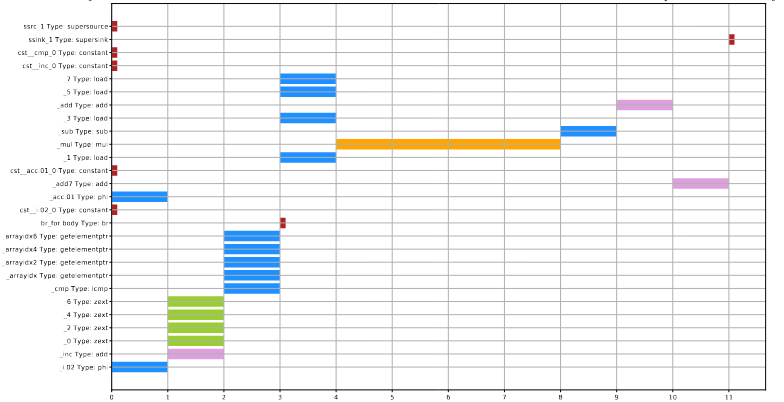
\includegraphics[width=.9\textwidth]{figures/kernel3_asap.png}
                    \caption{Kernel 3 with ASAP scheduling}
                    \label{fig:kernel3-asap}
            \end{figure}
            \begin{figure}[H]
            \centering
                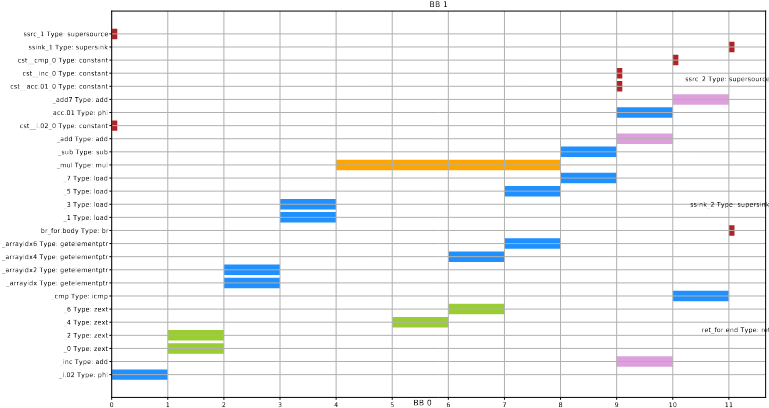
\includegraphics[width=.9\textwidth]{figures/kernel3_alap.png}
                \caption{Kernel 3 with ALAP scheduling}
                \label{fig:kernel3-alap}
            \end{figure}
            Scheduling more of the same operation in the same cycle means that more hardware is necessary to execute the schedule. In the case of kernel 3, ASAP scheduling causes cycle 1 to need 4 \emph{zext} hardware units to execute properly, as opposed to the 2 \emph{zext} units needed for ALAP. However, ASAP scheduling only needs 1 \emph{add} unit, compared to the 2 units needed with ALAP, so there is a small tradeoff to be made.
            \item Kernel 4: For this kernel, ASAP scheduling requires 5 \emph{add} units, while ALAP scheduling only needs 2.
        \end{itemize}
    \end{enumerate}
    \section{Task 4: ASAP with Resource Constraints}
    \begin{enumerate}
        \item
        \begin{itemize}
            \item Kernel 1:
            \begin{itemize}
                \item Setting the resource constraints to the lowest possible, i.e. \emph{\{'add': 1, 'mul': 1, 'zext': 1\}} causes the highest achievable latency of 16.
                \item Since there is only 1 \emph{add} operation and 3 \emph{mult} operations (of which maximum 2 can be scheduled at the same time). All resource constraints higher than \emph{\{'add': 1, 'mul': 2, 'zext': 1\}} lead to the same schedule. They all have a latency of 13.
            \end{itemize}
            \item Kernel 2:
            \begin{itemize}
                \item Because kernel 2 only has 2 \emph{mult} operations, with 0 slack each, meaning they can never be scheduled at the same time, as well as 0 \emph{add} and \emph{zext} operations, resource constraints have no impact on this kernel's ASAP schedule. The schedule therefore always has a latency of 10.
            \end{itemize}
            \item Kernel 3:
            \begin{itemize}
                \item Kernel 3 is the only kernel with \emph{zext} operations
                \item Setting the resource constraints to the lowest possible, i.e. \emph{\{'add': 1, 'mul': 1, 'zext': 1\}} causes the highest achievable latency of 16.
                \item Setting the resource constraints to the highest necessary, i.e. \emph{\{'add': 1, 'mul': 1, 'zext': 4\}} for this kernel, leads to the lowest achievable latency of 11.
            \end{itemize}
            \item Kernel 4:
            \begin{itemize}
                \item Setting the resource constraints to the lowest possible, i.e. \emph{\{'add': 1, 'mul': 1, 'zext': 1\}} causes the highest achievable latency of 27.
                \item Setting the resource constraints to the highest necessary, i.e. \emph{\{'add': 5, 'mul': 2, 'zext': 1\}} for this kernel, leads to the lowest achievable latency of 22.
            \end{itemize}
        \end{itemize}
        \item
        \begin{itemize}
            \item Kernel 1: As shown in Figure \ref{fig:kernel1-asap-rconst}, setting the resource constraints to a value larger or equal to the maximum number of needed resources, produces an identical schedule to ASAP without resource constraints
                \begin{figure}[H]
                    \centering
                    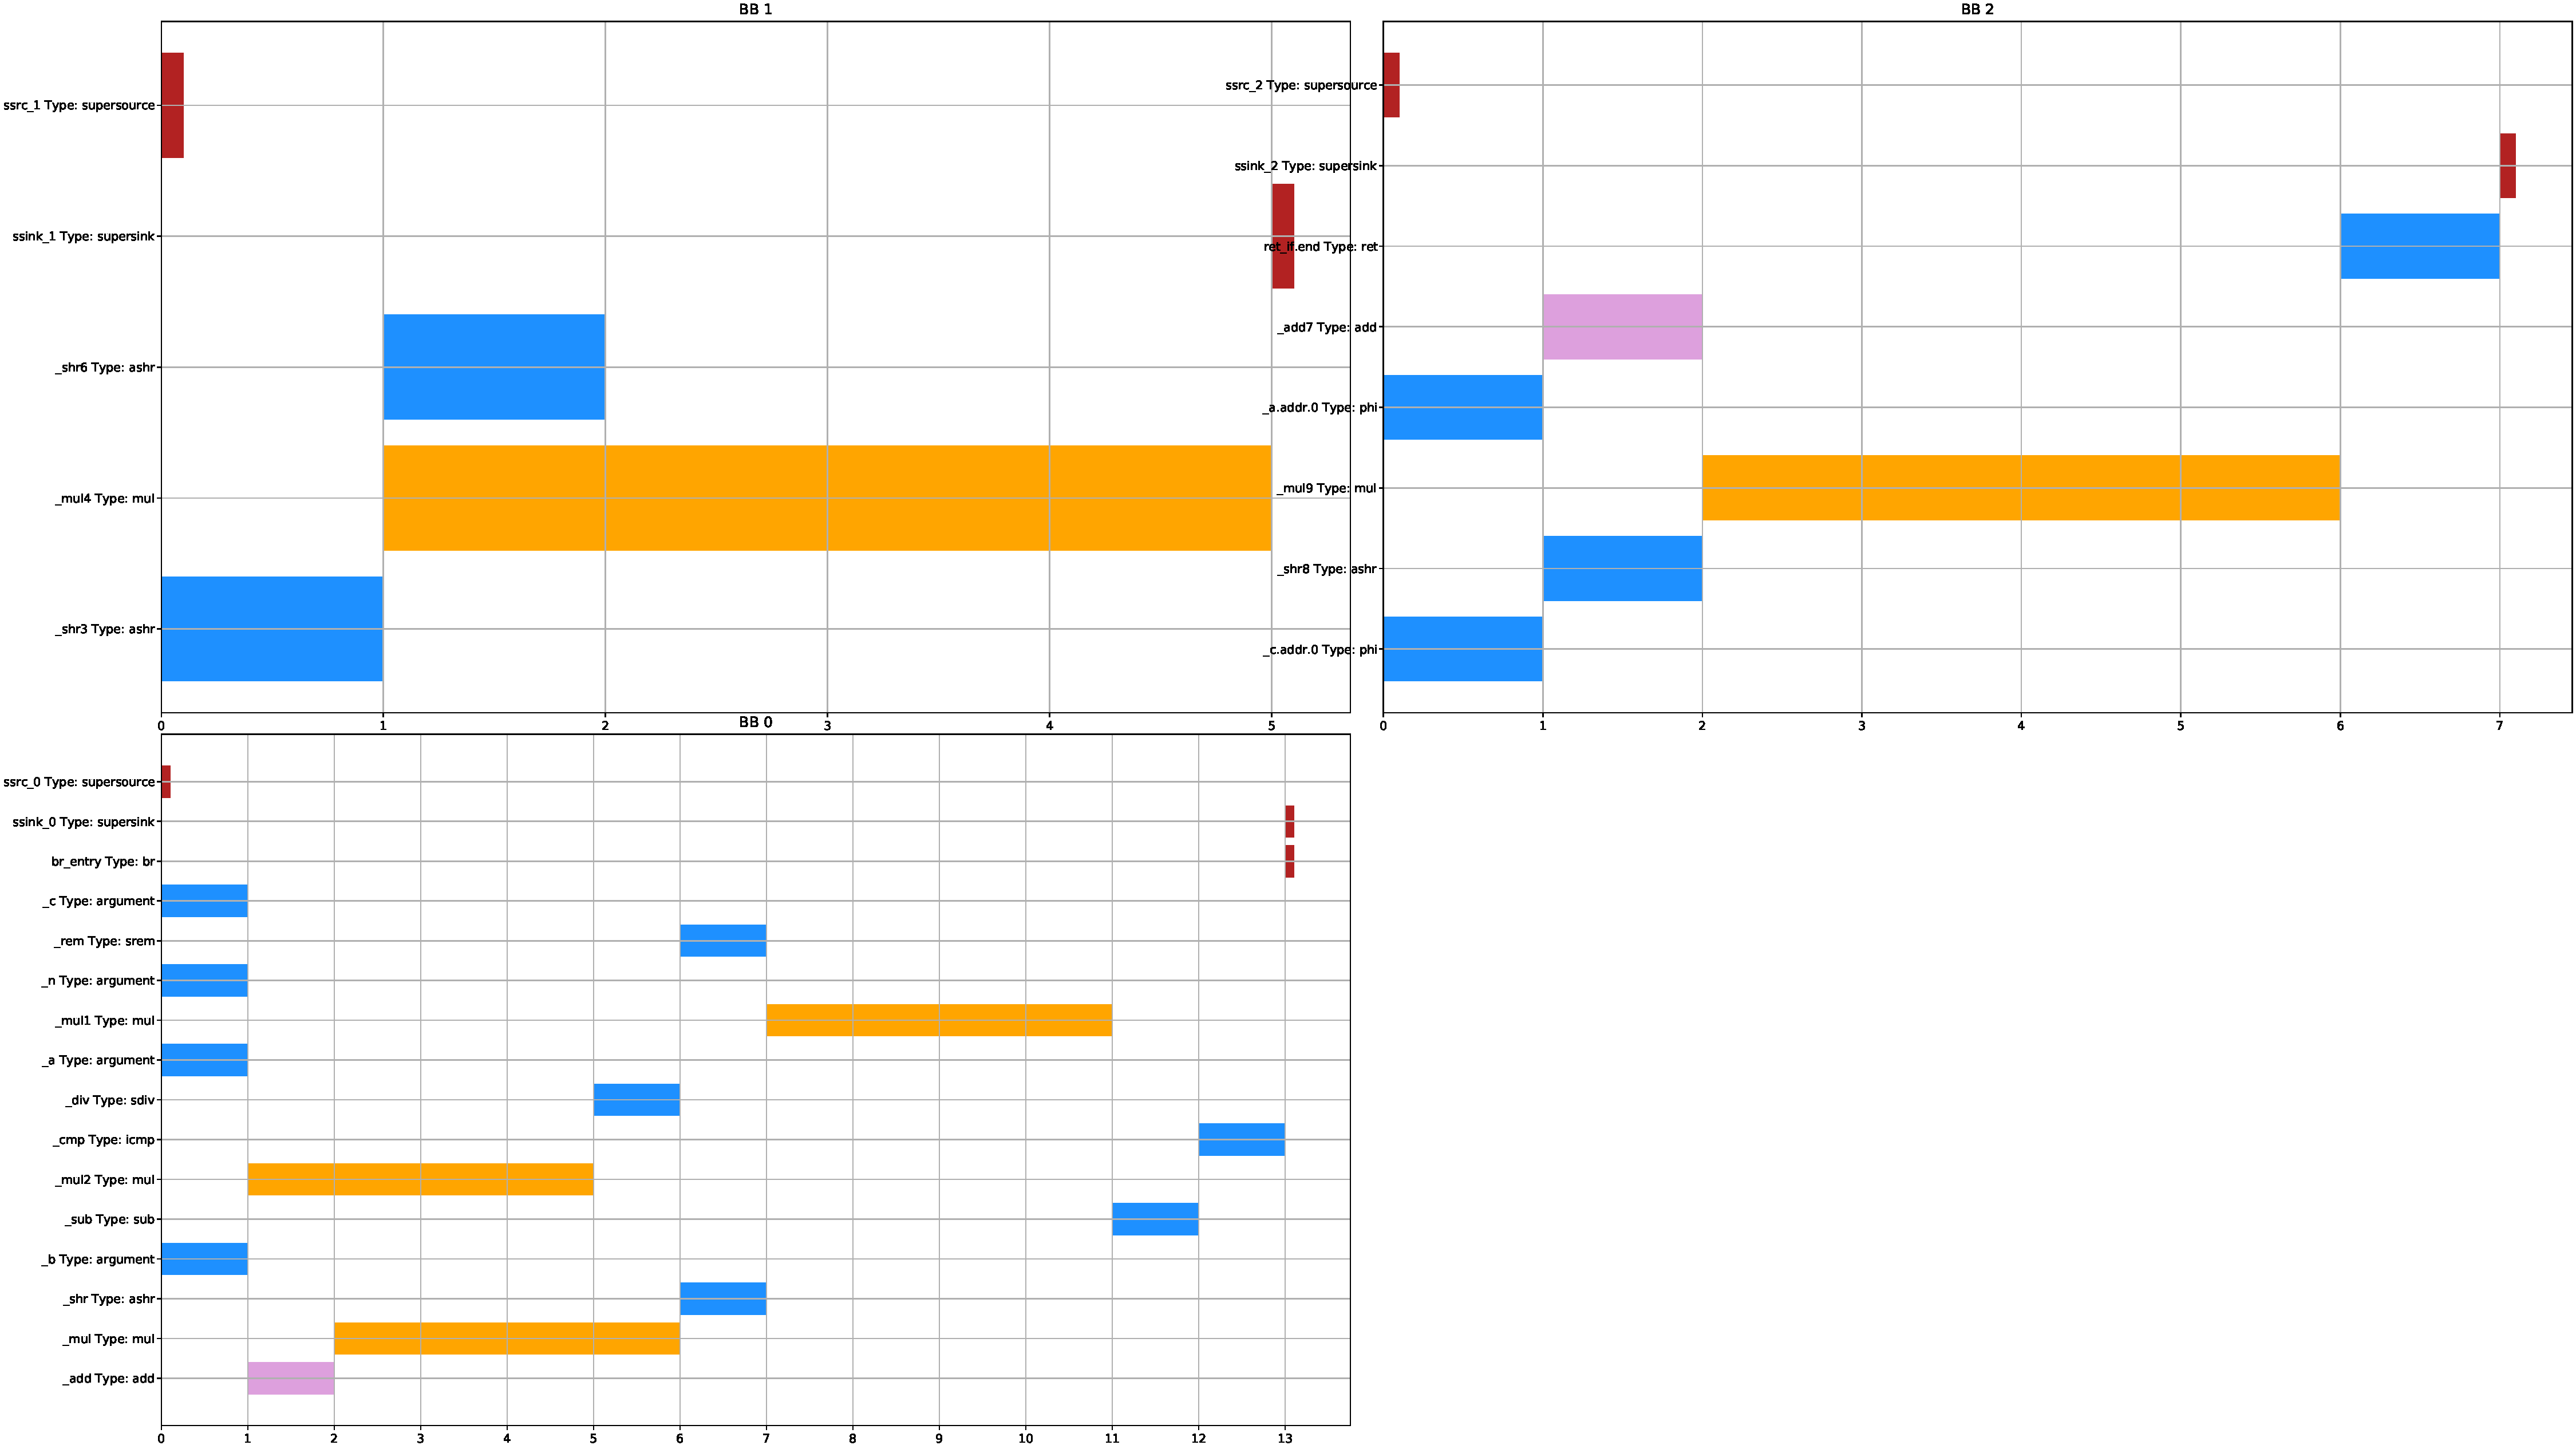
\includegraphics[width=0.9\textwidth]{figures/asap_kernel_1.pdf}
                    \caption{Kernel 1 with ASAP scheduling and resource constraints}
                    \label{fig:kernel1-asap-rconst}
                \end{figure}
            \item Kernel 2: Resource constraints have no impact on the schedule of this kernel, for reasons stated above.
            \item Kernel 3: For resource constraints \emph{\{'add': 1, 'mul': 1, 'zext': 4\}} (or higher), the schedule is the same as ASAP without constraints.
            \item Kernel 4: For resource constraints \emph{\{'add': 5, 'mul': 2, 'zext': 1\}} (or higher), the schedule is the same as ASAP without constraints.
        \end{itemize}
    \end{enumerate}
    \section{Task 5: Pipelined Schedule}
    \begin{enumerate}
        \item For N loop iterations, the total latency can be calculated as \[total\ latency = latency + (N-1)*II\] where $latency$ refers to the latency of 1 iteration. The total latencies of the kernels for N loop iterations as well as the required area are listed below.
        \begin{itemize}
            \item Kernel 1: $II = 1$ and $latency = 13$, $total\ latency = 13 + (N-1)$, required area: 1 \emph{add} and 2 \emph{mult} units
            \item Kernel 2: $II = 1$ and $latency = 10$, $total\ latency = 10 + (N-1)$,
            required area: 1 \emph{add} and 1 \emph{mult} units
            \item Kernel 3: $II = 2$ and $latency = 11$, $total\ latency = 11 + (N-1)*2$,
            required area: 1 \emph{add}, 1 \emph{mult} and 4 \emph{zext} units
            \item Kernel 4: $II = 19$ and $latency = 22$, $total\ latency = 22 + (N-1)*19$, required area: 5 \emph{add} and 2 \emph{mult} units
        \end{itemize}
        \item The achievable II's are listed above.
    \end{enumerate}
    \section{Task 6: Resource Constraints with Pipelining}
    \begin{enumerate}
        \item No, the MRT heuristic does not compute the optimal scheduling. This is the case because it uses a iterative approach which simply increases the \emph{II} until a valid MRT schedule is found. However, this method misses schedules where a slightly different arrangement of operations might be beneficial.
        \item The MRT heuristic suffers from the limitation that all operations of one iteration must be executed consecutively (without any NOPs in between). The upside to this limitation is that it is very easily computable and thus very efficient.
        \item The heuristic could be improved by also adding the possibility of adding NOPs in between operations or reordering the operations. However, this would lead to a much higher computational load and the MRT's efficiency would suffer greatly.
    \end{enumerate}
    
\end{document}